\documentclass[12pt,a4paper,openright,twoside]{book}
\usepackage[utf8]{inputenc}
\usepackage{disi-thesis}
\usepackage{code-lstlistings}
\usepackage{notes}
\usepackage{shortcuts}
\usepackage{acronym}
\usepackage{float}

\school{\unibo}
\programme{Corso di Laurea in Ingegneria e Scienze Informatiche}
\title{Monitoraggio Ed Automazione Della Distribuzione Di Software Complessi}
\author{Marco Sternini}
\date{\today}
\subject{Programmazione ad oggetti}
\supervisor{Dott. Danilo Pianini}
\cosupervisor{Dott.sa Martina Baiardi}
\session{III}
\academicyear{2022-2023}

% Definition of acronyms
\acrodef{vm}[VM]{Virtual Machine}
\acrodef{cicd}[CI/CD]{Continuous Integration Continuous Delivery}
\acrodef{cli}[CLI]{Command Line Interface}
\acrodef{jvm}[JVM]{Java Virtual Machine}
\acrodef{jre}[JRE]{Java Runtime Environment}
\acrodef{aur}[AUR]{Arch User Repository}
\acrodef{dsl}[DSL]{Domain-Specific Language}
\acrodef{kiss}[KISS]{Keep It Simple, Stupid}

\mainlinespacing{1.241} % line spacing in mainmatter, comment to default (1)

\begin{document}

\frontmatter\frontispiece

\begin{abstract}	
Max 2000 characters, strict.
\end{abstract}

\begin{dedication} % this is optional
Optional. Max a few lines.
\end{dedication}

\begin{acknowledgements} % this is optional
Optional. Max 1 page.
\end{acknowledgements}

%----------------------------------------------------------------------------------------
\tableofcontents   
\listoffigures     % (optional) comment if empty
\lstlistoflistings % (optional) comment if empty
%----------------------------------------------------------------------------------------

\mainmatter

%----------------------------------------------------------------------------------------
\chapter{Introduzione}
\label{chap:introduction}
%----------------------------------------------------------------------------------------

Introduzione 

(Il problema, software oggigiorno, l'importanza della qualità del software e altre caratteristiche di ingegneria del software, come automatizzare migliora la qualità eliminando l'intervento umano)

\section{Contesto}

(Un'introduzione teorica degli elementi sotto elencati, cosa servono, esempi di software che risolvono questo problema, evoluzione di questi negli ultimi anni )

\subsection{Build automation}
\subsection{Continuous integration}
\subsection{Continuous delivery}
\paragraph{Pipeline}

\subsection{Alchemist}

(Cos'è alchemist, utilizzo, tecnologie utilizzate, architettura, progettazione)

\section{Obiettivi}

\paragraph{Struttura della tesi}

La struttura di questo paper

\chapter{Analisi}

Il progetto si pone tre principali obiettivi:
\begin{itemize}
	\setlength\itemsep{0.8em}
	\item La generazione automatica di pacchetti di installazione multi-piattaforma \\ con \ac{jre} integrato
	\item La pubblicazione automatica di rilasci all'interno dell'\ac{aur}
	\item Lo sviluppo di una \ac{cli} per interagire con il simulatore
\end{itemize}

Con integrazione di un \ac{jre} si intende il supplemento di una \ac{jvm}, frequentemente ridotta di dimensioni, all'interno del pacchetto di installazione.
L'utente potrebbe non aver alcun \ac{jre} installato sul proprio dispositivo, oppure quello presente potrebbe essere obsoleto. Inserendo una macchina virtuale Java: si fornisce uno specifico ambiente di esecuzione eliminando potenziali problemi di compatibilità e si agevola la procedura di installazione per l'end-user. L'avvio dell'applicazione è delegato ad un file eseguibile nativo del sistema operativo ospitante.

\section{Requisiti}

\paragraph{Requisiti funzionali}

Le funzionalità richieste si possono classificare in due gruppi distinti: il primo contiene tutto ciò che concerne l'esperienza dell'utente finale, mentre il secondo descrive le funzionalità dal punto di vista degli sviluppatori e contributori di Alchemist. Di seguito il primo gruppo.
\begin{itemize}
	\item \textbf{Multi-piattaforma}: Alchemist deve essere installabile sui maggiori sistemi operativi in circolazione come Windows, MacOS e le principali distribuzioni Linux (Debian, Fedora, Arch).
	\item \textbf{Usabilità}: il simulatore deve fornire un'interfaccia \ac{cli} completa ed autoesplicativa, ossia che permetta l'utilizzo di tutte le sue funzionalità.
\end{itemize}

I requisiti del gruppo successivo sono accumunabili per il loro scopo, vale a dire l'automazione.

\begin{itemize}
	\item \textbf{Automazione dei pacchetti}: la generazione dei pacchetti di installazione deve essere automatica e configurabile
	\item \textbf{Automazione della distribuzione}: il rilascio di una nuova versione deve fornire i pacchetti all'interno di GitHub e pubblicare l'aggiornamento nell'\ac{aur}.
	\item \textbf{Verifica funzionamento}: entrambi i processi descritti precedentemente devono essere corredati da verifiche del loro funzionamento e devono bloccare la procedura di rilascio nell'eventualità siano presenti errori.
\end{itemize}

\paragraph{Requisiti non funzionali}

\begin{itemize}
	\item Trattandosi Alchemist di un software in continuo sviluppo, è auspicabile l'utilizzo degli strumenti già impiegati all'interno del repository. L'integrazione di nuovi applicativi deve essere eseguita solo se strettamente necessaria.
	\item La pipeline aggiornata deve assicurare tempi di esecuzione non maggiori alla versione precedente.
\end{itemize}

\section{Strumenti}

\subsection{Gradle}

Strumento open source di build automation configurabile attraverso due diversi \ac{dsl}: Groovy o Kotlin. Gradle utilizza un grafo aciclico diretto per determinare l'ordine di esecuzione dei processi. Un processo viene chiamato "task" e si tratta dell'unità di esecuzione più piccola configurabile. Gradle supporta lo sviluppo incrementale essendo capace di riconoscere quali task rieseguire a fronte di una modifica alla configurazione.
Il procedimento di build si divide in tre fasi distinte.
\begin{enumerate}
	\item \textbf{Fase di inizializzazione}. In primo luogo Gradle crea un istanza di Settings che organizza l'architettura del progetto. Attraverso un file, di nome "settings.gradle", lo sviluppatore stabilisce il progetto radice e tutti gli eventuali progetti figli. 
	\item \textbf{Fase di configurazione}. Successivamente tutti i file di configurazione build.gradle (del progetto radice e tutti i sotto-progetti) vengono analizzati per costruire il grafo dei task. Un task rappresenta un'unità atomica di esecuzione.
	\item \textbf{Fase di esecuzione}. Infine, Gradle esegue i task richiesti considerando le dipendenze descritte nel grafo generato dalla fase precedente.
\end{enumerate}
\subsection{GitHub actions}

GitHub Actions è una piattaforma di \ac{cicd} disponibile per i repository ospitati su GitHub. Permette di costruire ed automatizzare pipeline di build, test oppure distribuzione del software.

\paragraph{Componenti} 

\subsection{Arch User Repository}

\paragraph{Gestore pacchetti} Nei sistemi operativi Linux il controllo dei componenti installati nella macchina è completamente delegato ai \textit{package manager}. Il \textit{package-management system} è un insieme di strumenti software che gestiscono i processi di installazione, aggiornamento, configurazione e rimozione di applicativi dal sistema. Spesso un pacchetto corrisponde ad un particolare programma o applicazione. Allo stesso tempo però esistono applicativi più complessi composti da più pacchetti correlati. Il sistema di gestione dei pacchetti opera attraverso tre componenti principali.

\begin{itemize}
	\item Un componente a basso livello che si occupa dell'installazione o rimozione dei pacchetti.
	\item Un componente ad alto livello il cui compito principale è quello di fornire un'interfaccia per la gestione dei pacchetti all'utente. Si occupa inoltre di risolvere le dipendenze e gestire le sorgenti (repository).
	\item I repository, ossia database pubblici contenenti i pacchetti ed i relativi meta-dati.
\end{itemize}

\begin{figure}[H]
	\centering
	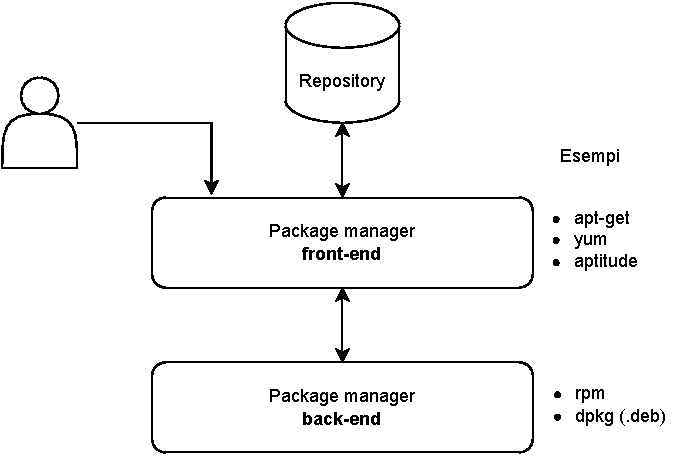
\includegraphics[width=.7\linewidth]{figures/package-managers.pdf}
	\caption{Struttura più diffusa dei sistemi di gestione di pacchetti}
	\label{fig:package-managers}
\end{figure}

\paragraph{Arch Linux} Una distribuzione importante nel vasto panorama dei fork Linux è Arch. Arch è una distribuzione Linux con architettura x86-64 creata seguendo la filosofia \ac{kiss}. È infatti rinomata per essere leggera, veloce, estremamente scalabile ed adattabile alle proprie esigenze. Data la sua natura minimalista, l'installazione iniziale non incorpora alcun strumento di configurazione automatica, nessun ambiente desktop e nessun altro strumento necessario all'avvio del sistema. Il sistema di gestione dei pacchetti si chiama \textit{pacman} ed a differenza dei concorrenti, opera sia a basso che ad alto livello. Un pacchetto non è altro che un file shell script denominato \textit{PKGBUILD} contenente le istruzioni necessarie a scaricare i sorgenti e compilarli attraverso un comando: \textit{makepkg}. La linearità dei file PKGBUILD rende la creazione di pacchetti alla portata di qualsiasi utente. \ac{aur} è una peculiarità di Arch che la distingue dalle altre distribuzioni. Si tratta di un repository di pacchetti in cui qualsiasi utente, anche non sviluppatore, può contribuire. 

\paragraph{Analisi rispetto ai requisiti}



\paragraph{Conclusioni}

\chapter{Design}

\section{Architettura e macrostruttura}
Interazione tra gradle e github actions, l’attuale struttura della pipeline di alchemist, le aggiunte che sono state fatte..

\section{Impacchettamento}
Discussione sulla scelta del software di packaging, vantaggi / svantaggi

\subsection{GraalVM}

\subsection{JPackage}

\subsection{Valutazioni}

\section{Flusso di rilascio}
Il processo del rilascio di una release nuova di alchemist, dalle automazioni già presenti alle integrazioni di testing, impacchettamento e pubblicazione
\subsection{Rilascio}

\subsection{Pubblicazione}

\section{User experience}
Discussione design della terza parte

\subsection{CLI e GUI}

\subsection{Design CLI}

\chapter{Implementazione}

\begin{itemize}
	\item Particolari design nell'interfaccia CLI
	\item Esempi
\end{itemize}

\chapter{Conclusioni}

\section{Sviluppi futuri}

%----------------------------------------------------------------------------------------
% BIBLIOGRAPHY
%----------------------------------------------------------------------------------------

\backmatter

\nocite{*} % comment this to only show the referenced entries from the .bib file

\bibliographystyle{alpha}
\bibliography{bibliography}

\end{document}